\chapter{Experimental Results}
\label{sec:results}

In this chapter, the performance of the driver assistance system is evaluated by comparing the value of quantitative properties in the human driver model obtained in Chapter~\ref{sec:human_driver} to similar properties in the model of the human driver with the ADAS designed in Chapter~\ref{sec:adas} (decision making with partially compliant drivers and with active linear acceleration and steering control). This is achieved using the various metrics defined throughout the dissertation, through random test cases of initial conditions and further comparison using a randomly generated sample population. After a discussion of the main results, some additional experiments regarding different properties outside the scope of the extensive comparison are presented.

\section{Human driver and ADAS comparison}

\subsection{Safety Results}
\label{sec:res_safety}

As initially described in Chapter~\ref{sec:human_driver}, the safety property for the human driver model can be written as:

\begin{minipage}{\linewidth}
{\vspace{1em}
\begin{lstlisting}
P=? [F crashed]
\end{lstlisting}
}
\end{minipage}

A similar safety property is presented in Chapter~\ref{sec:adas}, adapted for the fact that the model of the human driver and driver assistance system is an MDP instead of a DTMC:

\begin{minipage}{\linewidth}
{\vspace{1em}
\begin{lstlisting}
Pmin=? [F crashed]
\end{lstlisting}
}
\end{minipage}

These properties are directly comparable, as they represent the same quantitative value (this is not the case with the liveness properties). It should be noted that the lower the value of this property, the safer the system is. This means that these properties can be used not only for comparisons between the human driver alone and the full system (human and driver assistance system) for a given scenario, but also for inter-situational comparisons (i.e. with different initial conditions).

A scenario, in both cases, can be uniquely defined as a tuple $(d_{type}, v, v_1, x_{1,0})$, where $d_{type} \in \{1,2,3\}$ is the driver class considered (aggressive, average or cautious, respectively). In practice, this means that, for a road segment of $500m$ and considering $v, v_1 \in \{15,...,34\}$ and $x_{1,0} \in \{1,...,500\}$, there are $20 \times 20 \times 500 \times 3 = 600,000$ different scenarios to consider. Assuming that model checking each of those scenarios for both the human driver and the full system takes 5 minutes each (an assumption which will be challenged in Chapter~\ref{sec:conclusion}), this task would take approximately 2083 days to complete. Given the time frame of this dissertation, this would be infeasible. As such, three other methods where designed as a way to compare both systems: 

\begin{itemize}
	\item \textbf{Main vehicle initial velocity test cases}: for two randomly selected tuples $(v_1, x_{1,0})$, the variation of the value of the safety properties for each driver profile with the variation of $v$ were obtained. This directly compares 20 different scenarios for each driver class. The two tuples were randomly generated as $(v_1, x_{1,0}) = (20, 35)$ and $(v_1, x_{1,0}) = (22, 40)$, and the results are presented in Figures~\ref{fig:plot1} and \ref{fig:plot2}, respectively.
	\item \textbf{Bivariant initial velocity test cases}: for a randomly selected $x_{1,0}$, the variation of the values of the safety properties for each driver profile with the change of $v$ and $v_1$ (within certain ranges; $v \in \{20,...,30\}$ and $v_1\in \{15,...,25\}$) were generated. This directly compares 120 different scenarios for each driver class. The value $x_{1,0} = 50$ was randomly generated for this test case, and the results are presented in Figure~\ref{fig:plot3}.
	\item \textbf{Box plots}: for a randomly generated sample of 100 different initial conditions of $(v, v_1, x_{1,0})$, a box plot which represents the distribution of the values of the safety properties for this sample and for each driver profile was obtained. The results are shown in Figure~\ref{fig:plot6}.
\end{itemize}

\begin{figure}[H]
\centering
\begin{subfigure}{0.75\textwidth}
  \centering
  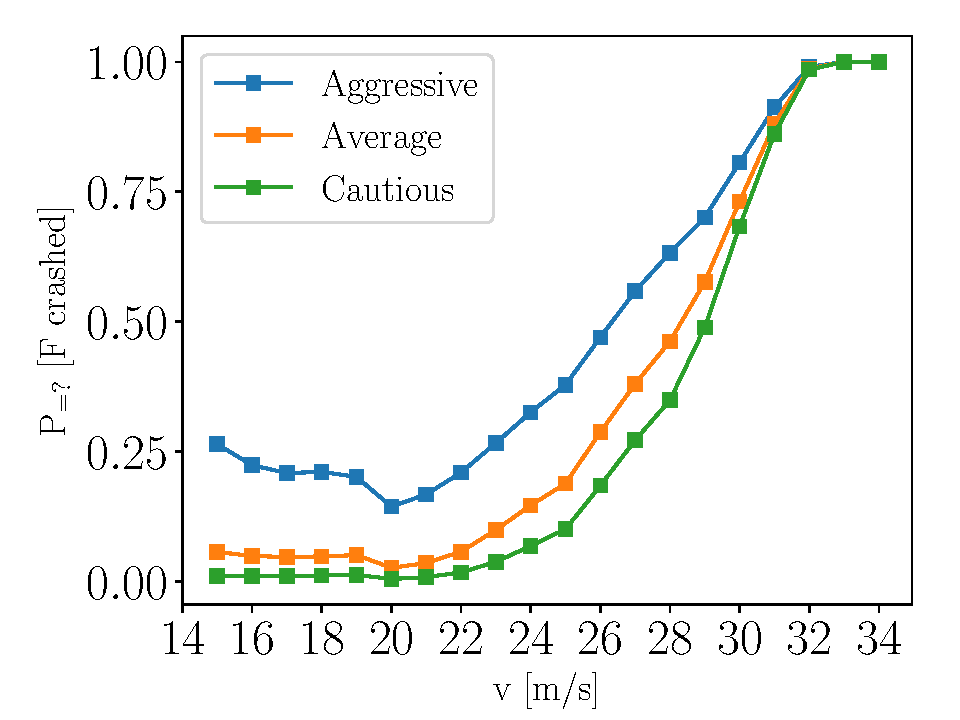
\includegraphics[width=1\textwidth]{results/safety/plot1_1.pdf}
  \subcaption{Human driver model}
\end{subfigure}
\begin{subfigure}{0.75\textwidth}
  \centering
  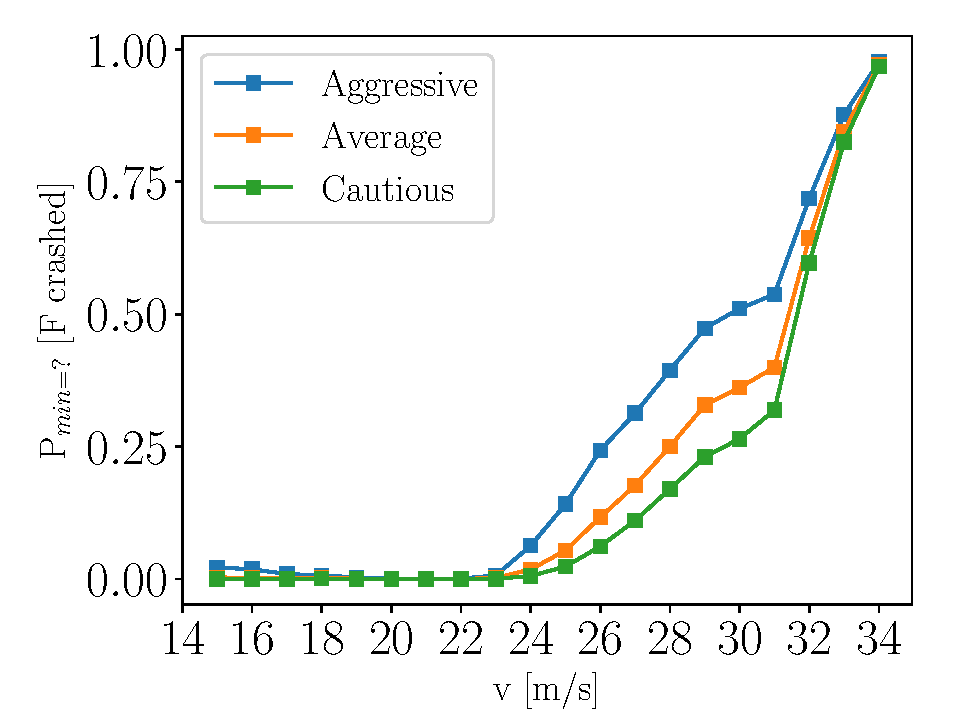
\includegraphics[width=1\textwidth]{results/safety/plot1_2.pdf}
  \subcaption{ADAS}
\end{subfigure} 
\caption{Plots of the variation of the value of the safety property with the initial velocity of the main vehicle for the conditions $v_1 = 20m/s$ and $x_{1,0} = 35m$.}
\label{fig:plot1}
\end{figure}

\begin{figure}[H]
\centering
\begin{subfigure}{0.75\textwidth}
  \centering
  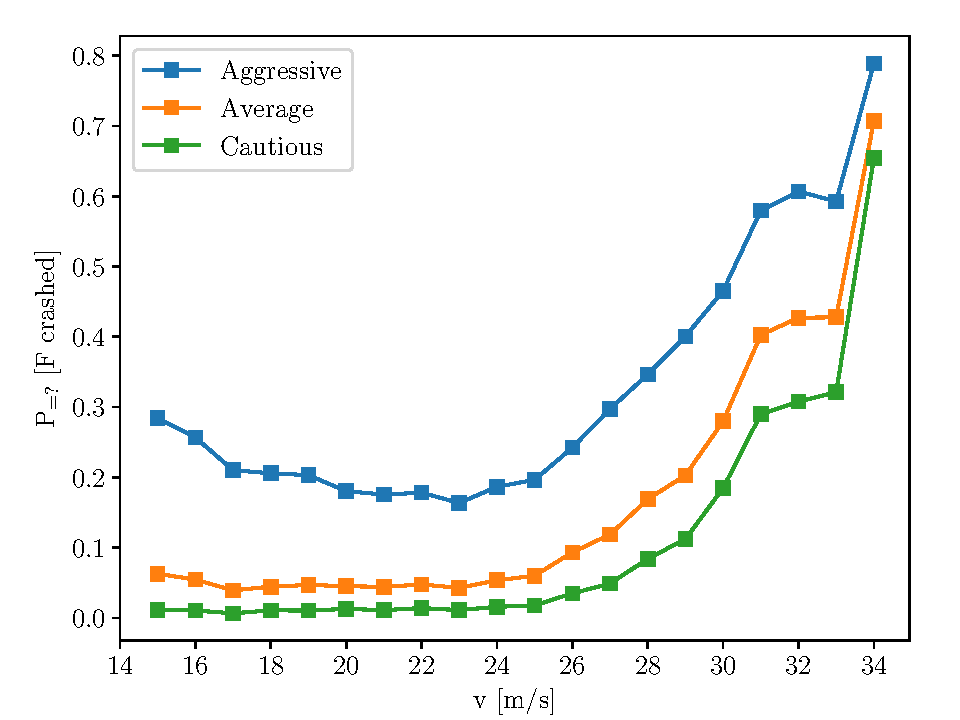
\includegraphics[width=1\textwidth]{results/safety/plot2_1.pdf}
  \subcaption{Human driver model}
\end{subfigure}
\begin{subfigure}{0.75\textwidth}
  \centering
  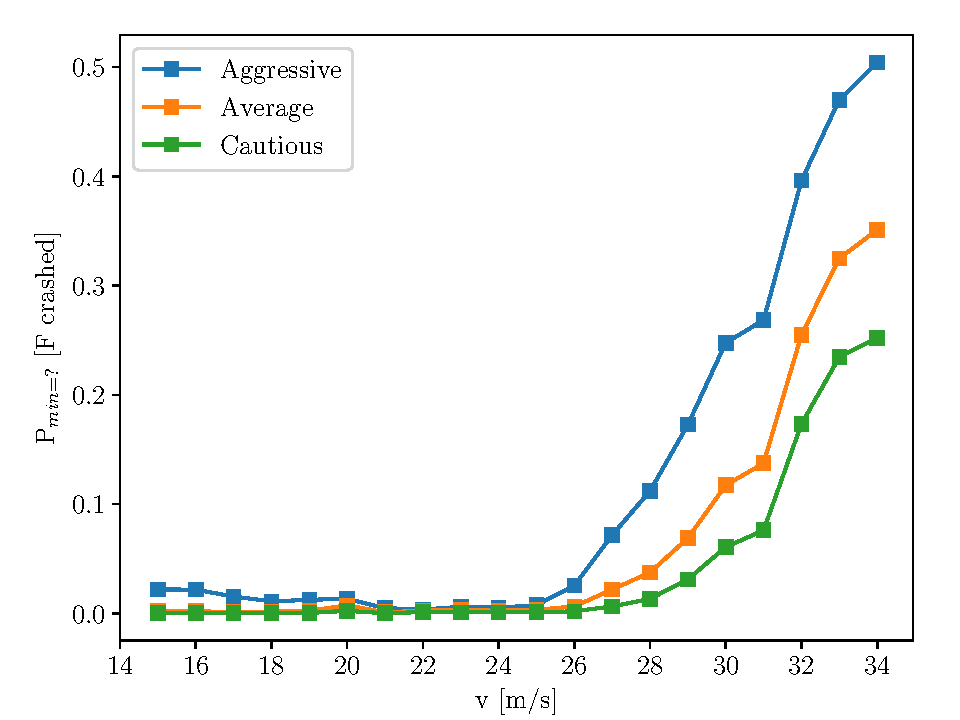
\includegraphics[width=1\textwidth]{results/safety/plot2_2.pdf}
  \subcaption{ADAS}
\end{subfigure} 
\caption{Plots of the variation of the value of the safety property with the initial velocity of the main vehicle for the conditions $v_1 = 22m/s$ and $x_{1,0} = 40m$.}
\label{fig:plot2}
\end{figure}

\begin{figure}[H]
\centering
\begin{subfigure}{0.5\textwidth}
  \centering
  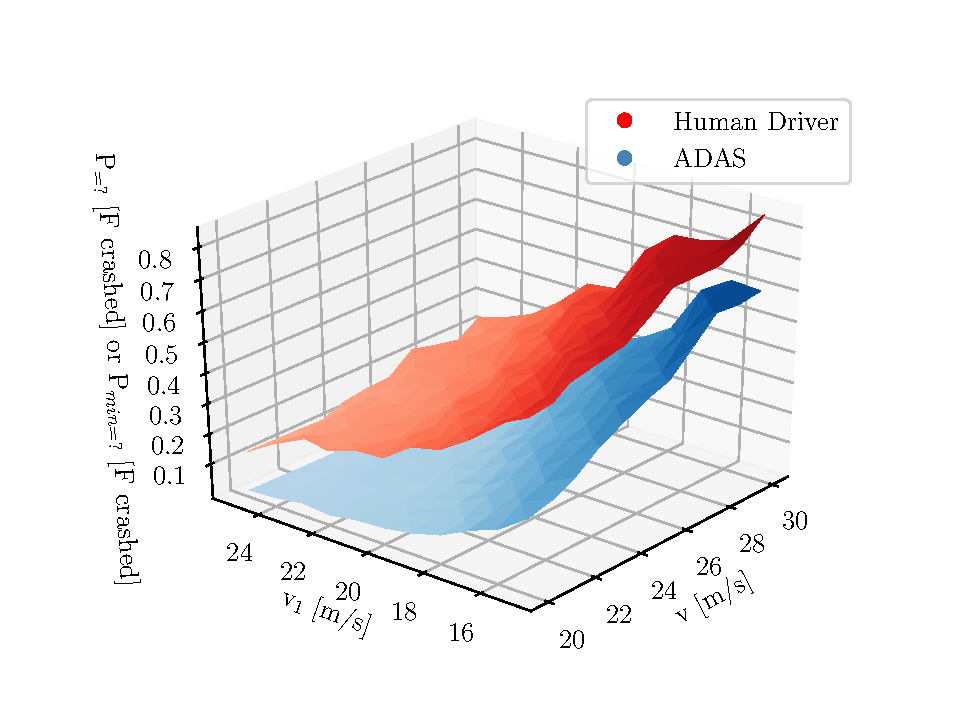
\includegraphics[width=1\textwidth]{results/safety/plot3_aggressive.pdf}
  \subcaption{Aggressive drivers}
\end{subfigure}
\begin{subfigure}{0.5\textwidth}
  \centering
  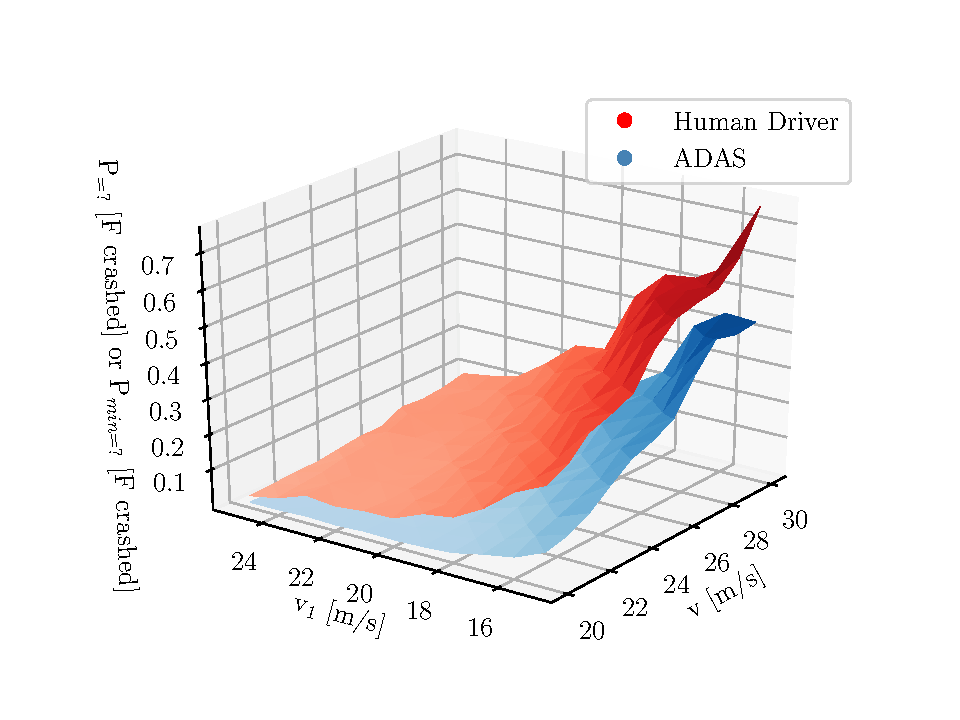
\includegraphics[width=1\textwidth]{results/safety/plot3_average.pdf}
  \subcaption{Average drivers}
\end{subfigure} 
\begin{subfigure}{0.5\textwidth}
  \centering
  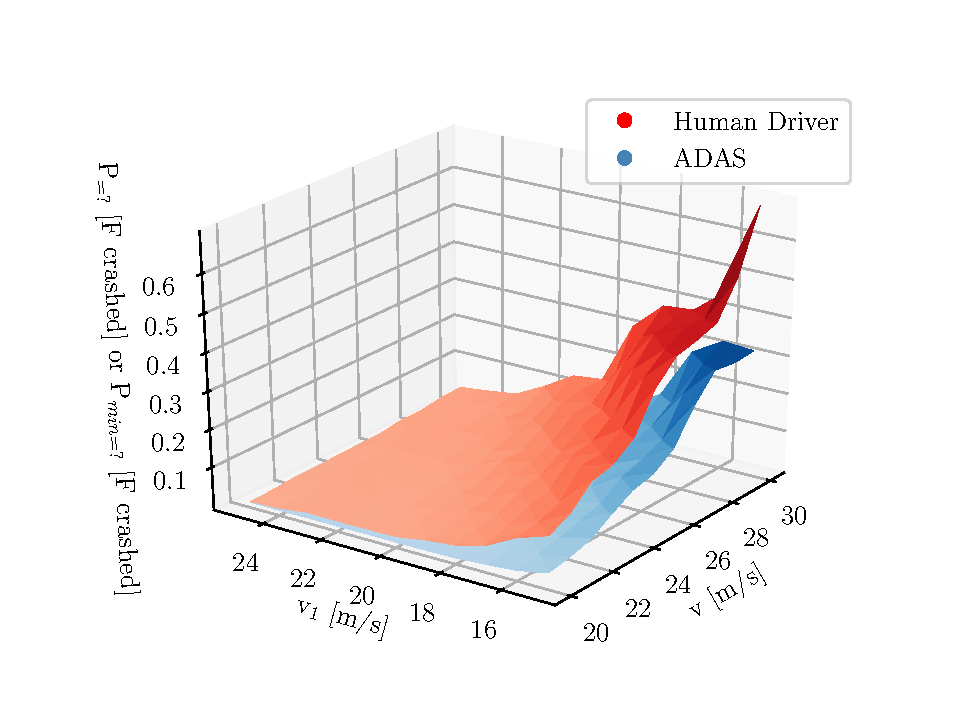
\includegraphics[width=1\textwidth]{results/safety/plot3_cautious.pdf}
  \subcaption{Cautious drivers}
\end{subfigure} 
\caption{Variation of the value of the safety properties with the initial velocities of both vehicles for $x_{1,0} = 50m$.}
\label{fig:plot3}
\end{figure}

\begin{figure}[H]
\centering
\begin{subfigure}{0.75\textwidth}
  \centering
  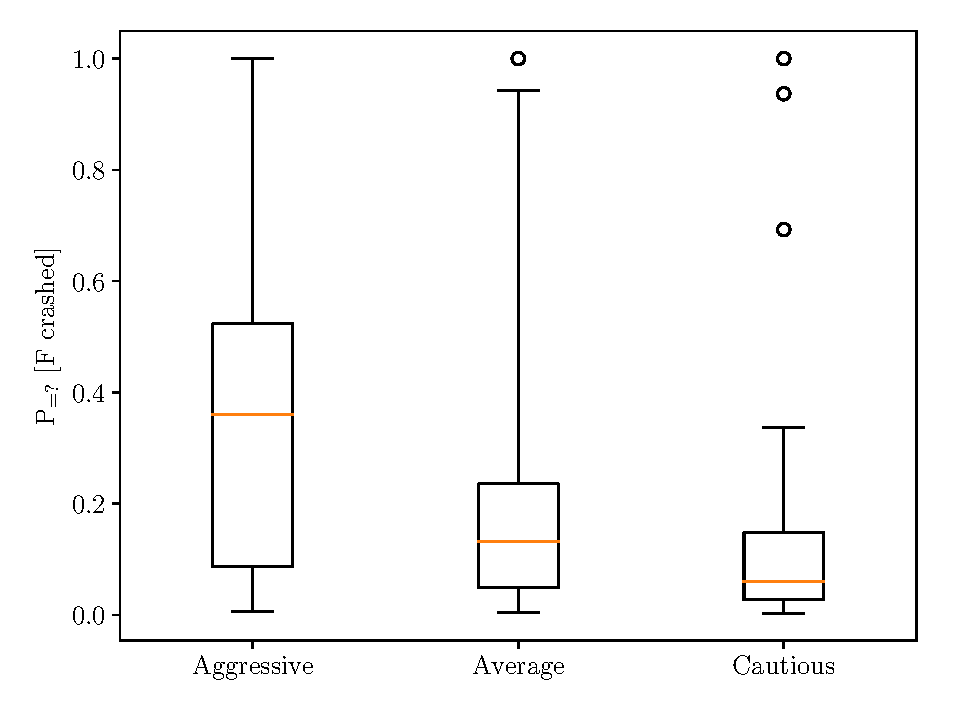
\includegraphics[width=1\textwidth]{results/safety/plot6_1.pdf}
  \subcaption{Human driver model}
\end{subfigure}
\begin{subfigure}{0.75\textwidth}
  \centering
  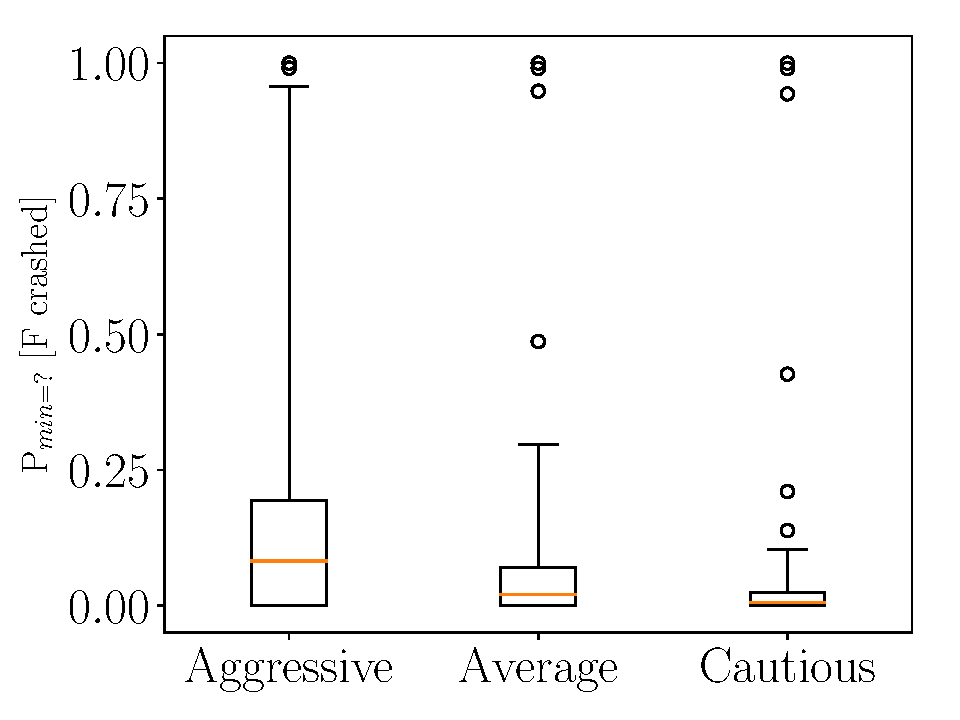
\includegraphics[width=1\textwidth]{results/safety/plot6_2.pdf}
  \subcaption{ADAS}
\end{subfigure} 
\caption{Box plot of the value of the safety properties for a randomly sampled population of 100 different initial conditions (equal in both cases).}
\label{fig:plot6}
\end{figure}

\subsection{Liveness Results}
\label{sec:res_liveness}

As introduced in Chapter~\ref{sec:human_driver}, there are multiple liveness properties that can be considered when evaluating the human driver model. However, the most appropriate ones for inter-situational comparisons are the conditional properties of the type:

\begin{minipage}{\linewidth}
{\vspace{1em}
\begin{lstlisting}
P=? [F (x=length) & (t<T) || F (x=length)]
\end{lstlisting}
}
\end{minipage}

for a given constant $T$.

In the case of the full system (human driver and ADAS), the model becomes an MDP and, as mentioned in Chapter~\ref{sec:background}, conditional properties are not so easily calculated in MDPs due to the existence of multiple adversaries. Despite this, it is possible to reason over lower bounds of these types of properties under the conditions of Proposition~\ref{pro:cond_props}. For the PCTL formulas $\varphi_1 = $\texttt{ F (x=length) \& (t<T)} and $\varphi_2 = $\texttt{ F (x=length)}, it is trivial that for any path $\pi \in Paths(s)$: $\pi \models \varphi_1 \Rightarrow \pi \models \varphi_2$. Furthermore, it can also be assumed that for:

\begin{equation}
	\sigma' \in \arg\sup_{\sigma \in Adv} P^{\sigma}_s (\varphi_1 \bigmid \varphi_2)
\end{equation}

it is true that:

\begin{equation}
	P^{\sigma'}_s (\varphi_1) = p_{\max, s} (\varphi_1)
\end{equation}

since intuitively the interest is in adversaries which maximise the conditional property through the maximisation of the probability of eventually reaching \texttt{(x=length) \& (t<T)} (as this is the comparable case in the human driver model). Thus, under the conditions of Proposition~\ref{pro:cond_props}, it is possible to write:

\begin{equation}
	p_{\max, s} (\text{\texttt{F (x=length) \& (t<T)}} \bigmid \text{\texttt{F (x=length)}}) \geq \frac{p_{\max, s} (\text{\texttt{F (x=length) \& (t<T)}})}{p_{\max, s} (\text{\texttt{F (x=length)}})}
\end{equation}

Therefore, a lower bound on the conditional probability, $\zeta$, can be obtained using the quantitative properties:

\begin{equation}
	\zeta = \frac{\text{\texttt{Pmax=? [F (x=length) \& (t<T)]}}}{\text{\texttt{Pmax=? [F (x=length)]}}}
\end{equation}

At this point it should also be noted that (as described in Section~\ref{sec:multi_obj_metrics}):

\begin{equation}
	p_{\max,s} (\text{\texttt{F x=length}}) = 1 - p_{\min,s} (\text{\texttt{F crashed}})
\end{equation}

so long as $p_{\max, s} (\text{\texttt{F (crashed | x = length)}}) = p_{\min, s} (\text{\texttt{F (crashed | x = length)}}) = 1$ (completeness property for the MDP). Therefore, $\zeta$ can be re-written as:

\begin{equation}
	\zeta = \frac{\text{\texttt{Pmax=? [F (x=length) \& (t<T)]}}}{1 - \text{\texttt{Pmin=? [F crashed]}}}
\end{equation}

As was the case with the safety properties, model checking the entire space of possible initial conditions would be infeasible given the time frame of this dissertation. Similarly, two methods were designed to compare both systems at the liveness level:

\begin{itemize}
	\item \textbf{Temporal variation of liveness}: for two randomly selected tuples $(v, v_1, x_{1,0})$, the value of all the pertinent liveness properties ($T \in \{16,...,28\}$) was obtained. The two tuples were randomly generated as $(v, v_1, x_{1,0}) = (21, 19, 70)$ and $(v, v_1, x_{1,0}) = (26, 22, 46)$, and the results are presented in Figures~\ref{fig:plot4} and \ref{fig:plot5}, respectively.
	\item \textbf{Box plots}: for a randomly generated sample of 100 different initial conditions of $(v, v_1, x_{1,0})$, obtain box plot which represents the distribution of the values of two liveness properties using appropriate values of $T$ (given the sample) for this sample and for each driver profile. After the sample was generated, it was determined that $T=21$ and $T=22$ were representative values (in the sense that they are great enough to avoid a significant portion of the values of both properties being 0, and not so large that a significant portion of the values for all scenarios are 1; these situations would make it impossible to compare the human and the full system). The results are presented in Figures~\ref{fig:plot7} and \ref{fig:plot8} for $T=21$ and $T=22$, respectively.
\end{itemize}

\begin{figure}[H]
\centering
\begin{subfigure}{0.75\textwidth}
  \centering
  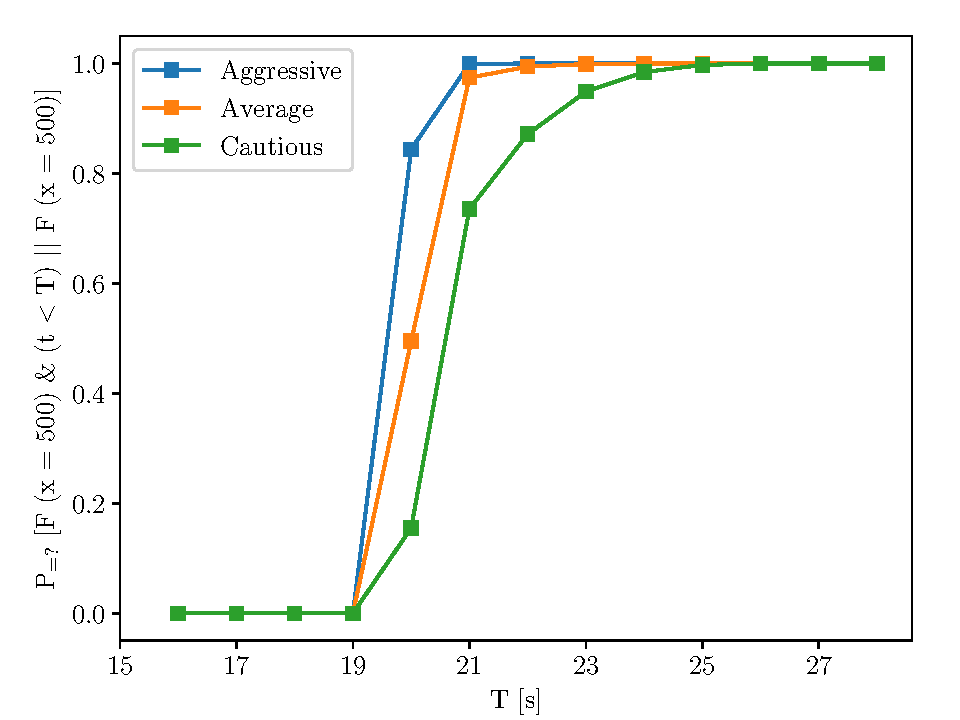
\includegraphics[width=1\textwidth]{results/liveness/plot4_1.pdf}
  \subcaption{Human driver model}
\end{subfigure}
\begin{subfigure}{0.75\textwidth}
  \centering
  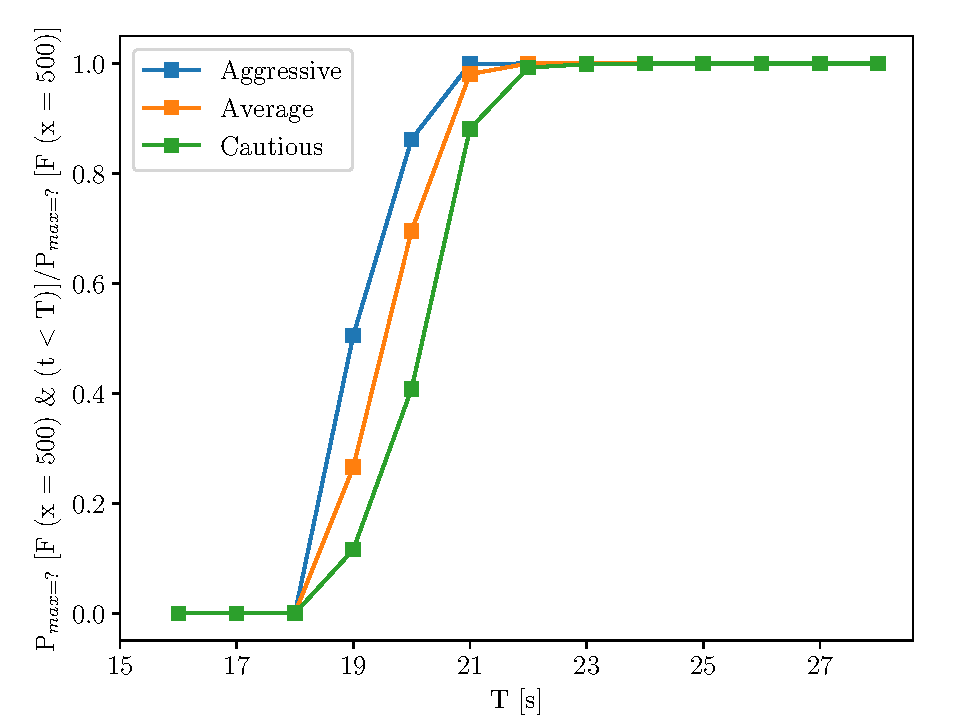
\includegraphics[width=1\textwidth]{results/liveness/plot4_2.pdf}
  \subcaption{ADAS}
\end{subfigure} 
\caption{Plots of the variation of the value of the liveness properties with the value of $T$ (in $s$) for the initial conditions $v = 21m/s$, $v_1 = 19m/s$ and $x_{1,0} = 70m$.}
\label{fig:plot4}
\end{figure}

\begin{figure}[H]
\centering
\begin{subfigure}{0.75\textwidth}
  \centering
  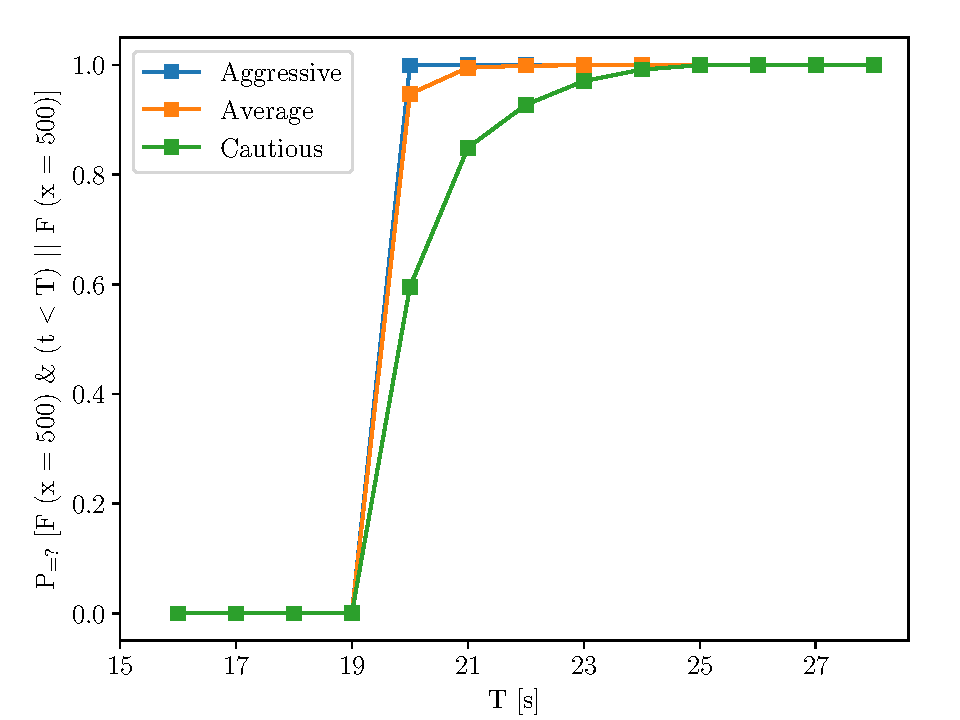
\includegraphics[width=1\textwidth]{results/liveness/plot5_1.pdf}
  \subcaption{Human driver model}
\end{subfigure}
\begin{subfigure}{0.75\textwidth}
  \centering
  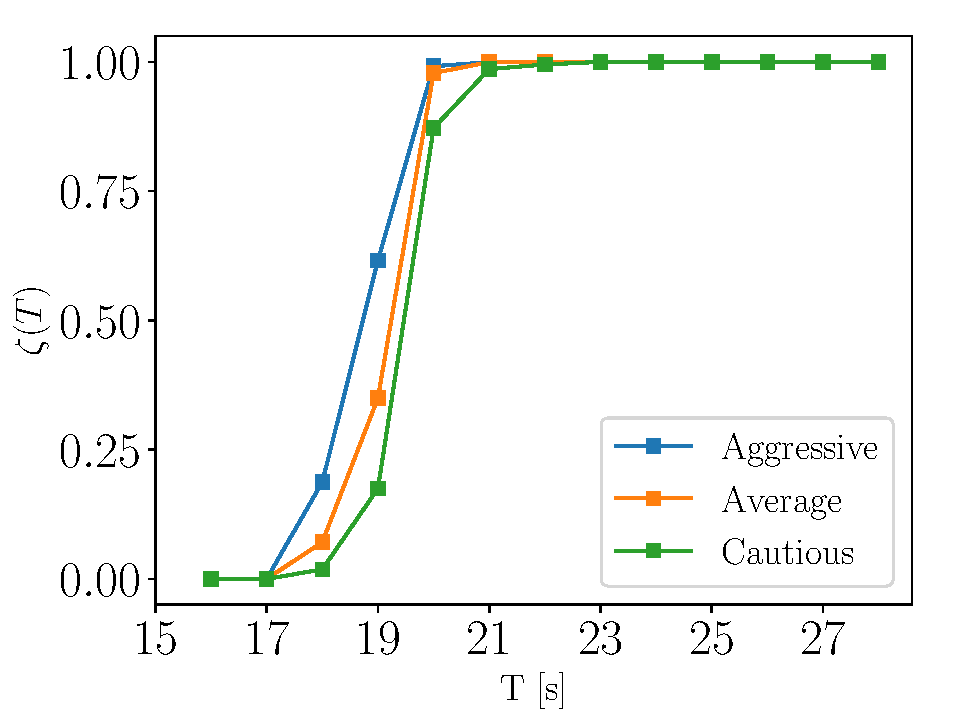
\includegraphics[width=1\textwidth]{results/liveness/plot5_2.pdf}
  \subcaption{ADAS}
\end{subfigure} 
\caption{Plots of the variation of the value of the liveness properties with the value of $T$ (in $s$) for the initial conditions $v = 26m/s$, $v_1 = 22m/s$ and $x_{1,0} = 46m$.}
\label{fig:plot5}
\end{figure}

\begin{figure}[H]
\centering
\begin{subfigure}{0.75\textwidth}
  \centering
  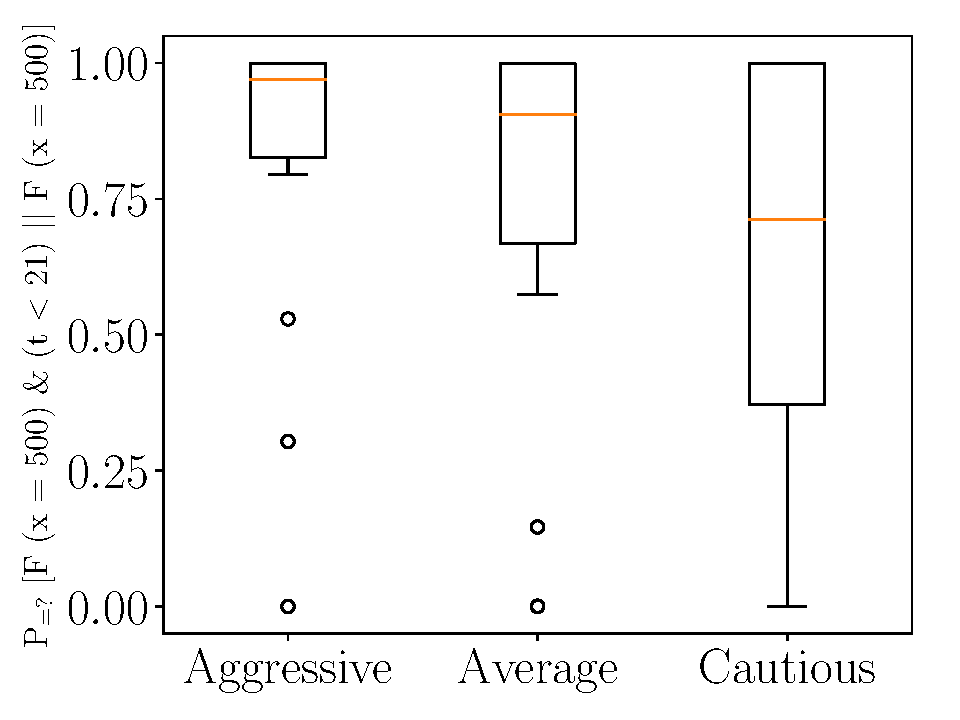
\includegraphics[width=1\textwidth]{results/liveness/plot7_1.pdf}
  \subcaption{Human driver model}
\end{subfigure}
\begin{subfigure}{0.75\textwidth}
  \centering
  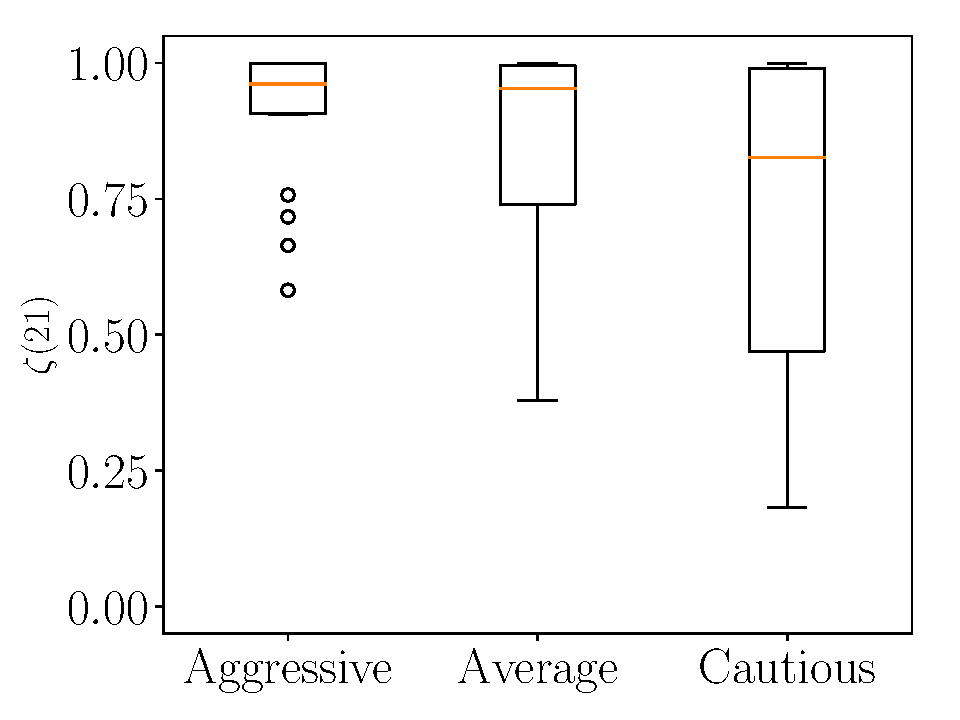
\includegraphics[width=1\textwidth]{results/liveness/plot7_2.pdf}
  \subcaption{ADAS}
\end{subfigure} 
\caption{Box plot of the value of the liveness properties for $T = 21s$ for a randomly sampled population of 50 different initial conditions (equal in both cases).}
\label{fig:plot7}
\end{figure}

\begin{figure}[H]
\centering
\begin{subfigure}{0.75\textwidth}
  \centering
  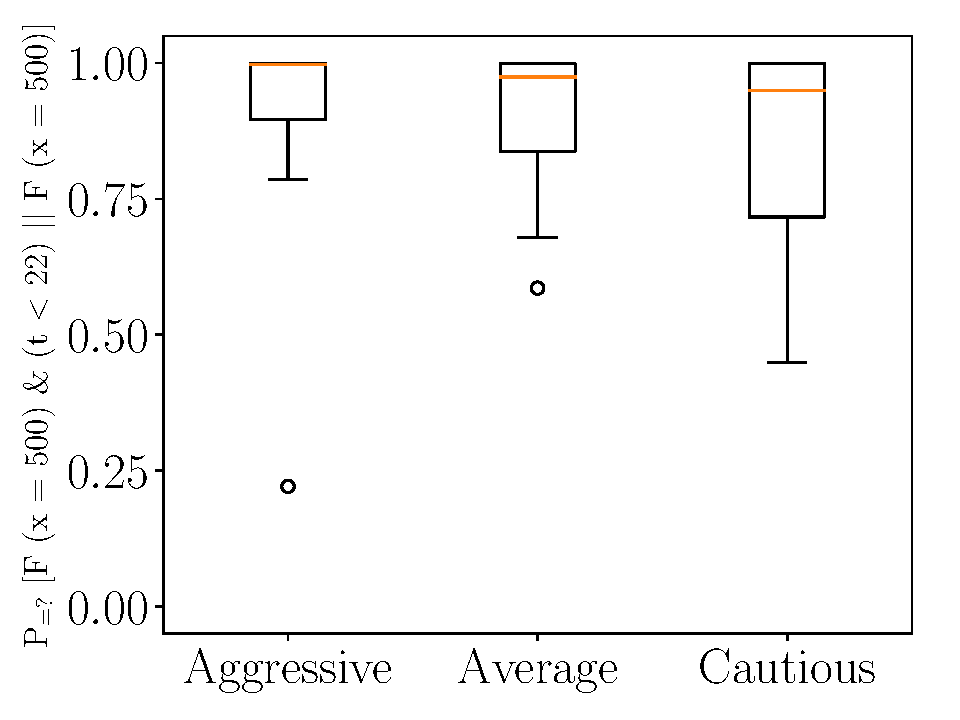
\includegraphics[width=1\textwidth]{results/liveness/plot8_1.pdf}
  \subcaption{Human driver model}
\end{subfigure}
\begin{subfigure}{0.75\textwidth}
  \centering
  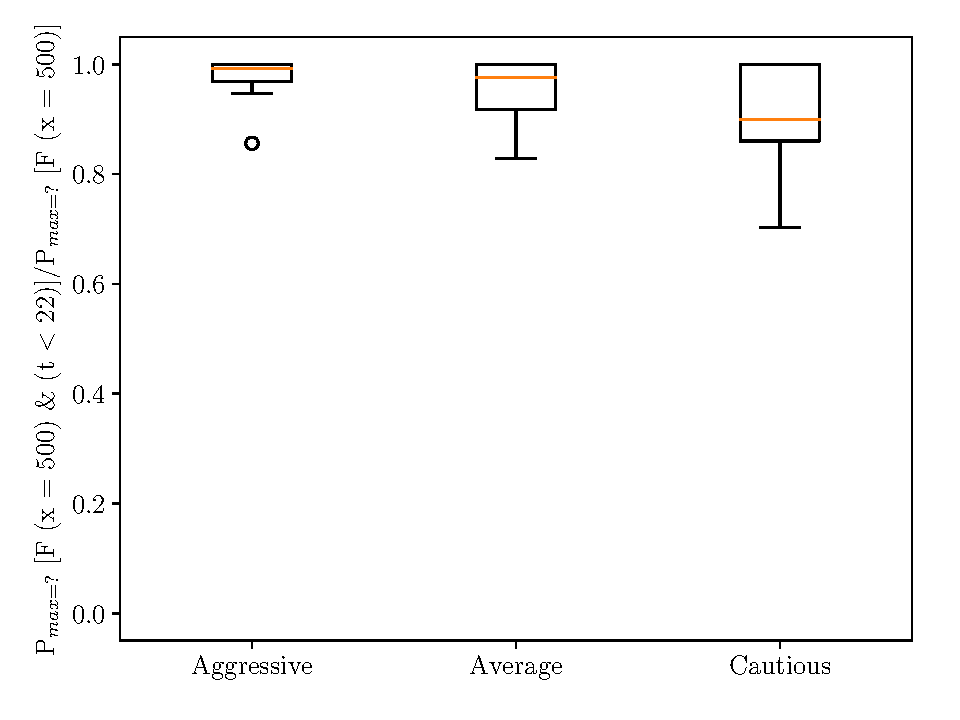
\includegraphics[width=1\textwidth]{results/liveness/plot8_2.pdf}
  \subcaption{ADAS}
\end{subfigure} 
\caption{Box plot of the value of the liveness properties for $T = 22s$ for a randomly sampled population of 50 different initial conditions (equal in both cases).}
\label{fig:plot8}
\end{figure}

\subsection{Discussion}

The discussion of the results presented in Sections~\ref{sec:res_safety} and \ref{sec:res_liveness} is threefold in nature. Firstly, the comparison between the different driver classes within each of the individual systems (i.e. human driver model and the human and ADAS system) is presented. Secondly, the results of the experiments of the human driver alone and the full system in both safety and liveness are discussed and compared (within the same driver profile). Finally, an overall discussion is presented on the extent of the validity of such comparisons through the drawbacks of the metrics used.

With respect to the individual driver classes presented in both the human driver model and the human and ADAS system, the results overwhelmingly support the initial idea that aggressive drivers perform the worse in terms of the safety metrics, followed by average drivers and finally cautious ones. While this is observable in the individual test cases (Figures~\ref{fig:plot1} and \ref{fig:plot2}), Figure~\ref{fig:plot6} firmly supports this conclusion within both systems. In terms of liveness, the reverse is true, with aggressive drivers outperforming average drivers who in turn outperform cautious drivers. Once more, while individual test cases support this result (Figures~\ref{fig:plot4} and \ref{fig:plot5}), Figures~\ref{fig:plot7} and \ref{fig:plot8} emphatically reinforce it. Intuitively, this is what was expected from the construction of the human driver model, and it is still noticeable even using the ADAS designed.

In terms of the comparison between the human driver model and the driver with the ADAS system, it becomes necessary to interpret the plots while considering the differences in the metrics used. 

In the safety evaluation, as mentioned in Section~\ref{sec:res_safety}, the results are directly comparable as the metrics are the equivalent of one another for the representation of the models of both systems (i.e. a DTMC for the human driver model and an MDP for the human and ADAS system). The most useful comparison in terms of the test cases in this metric is presented in Figure~\ref{fig:plot3}, as the 3D plots are divided into the three categories of drivers considered. It is observable that the introduction of the ADAS increases safety for all situations considered in this test case (i.e. reduces the value of the safety property). From the more general overview seen in Figures~\ref{fig:plot7} and \ref{fig:plot8}, the same conclusion is drawn for each driver class, with the $25\%$, $50\%$ (median) and $75\%$ quartiles being lower for the system with the ADAS than those for the human driver alone. 

With respect to liveness, the comparison needs to be carefully drawn, as the conditional property in the human driver model alone (DTMC) is not the equivalent of the metric chosen for liveness in the human and ADAS system (MDP). However, $\zeta$ is proven to be the lower bound of the conditional property in the human and ADAS system under the conditions presented in Section~\ref{sec:res_liveness}. From Figures~\ref{fig:plot4} and \ref{fig:plot5}, it can be observed that, for each $T$, the values of $\zeta$ are always greater or equal than those of the conditional property of the human driver model. The same result can be seen in Figures~\ref{fig:plot7} and \ref{fig:plot8} for $T=21$ and $T=22$, respectively, for the $25\%$ and $75\%$ quartiles. Given that $\zeta$ is the lower bound of the maximal conditional property, it can be concluded that the system with the ADAS outperforms the human driver alone in this metric. 

Despite the results pointing to the improvements in terms of the safety and liveness properties the ADAS designed brings, they should be taken with care, as there are drawbacks in the metrics used. 

The first drawback has to do with the fact that the comparison in the human and ADAS deals with minimal and maximal properties due to the existence of adversaries in MDPs. Thus, the fact that the safety property is lower in this case than in the human driver model and the liveness properties are higher, does not mean that there is a feasible strategy where both safety and liveness are optimal and outperform the human driver (there might be a trade-off). This is not the case with the human driver model, where it is known that both quantitative properties are satisfied simultaneously. In order to evaluate this feasibility properly, Pareto curves should be generated for each individual scenario and it should be seen whether there exists a Pareto point where both values outperform the human driver. This analysis is time consuming with the tools currently available (i.e. PRISM and Storm) and was therefore infeasible in the time frame of this dissertation. 

An additional drawback in terms of the liveness properties in the full system (i.e. human driver and ADAS system) case is that these are defined as lower bounds which are not proven to be tight. In fact, in Figure~\ref{fig:plot8}, while the $25\%$ and $75\%$ quartiles appear to be higher in the case of the full system than the human driver model, this is not the case with the median, which is at similar values (or even lower for the class of cautious drivers). From the rest of the data, it would appear that this value might be the result of the fact that the lower bound is not tight and might be underestimating the value of the maximal conditional property for the sample population used. However, this is not certain, and it might also be that the full system is outperformed, in terms of the liveness properties, by the human driver in certain conditions. The use of the unconditional liveness properties here would be meaningless, as it would incur in the safety bias first presented in Section~\ref{sec:live_props}. A solution to this problem would be to develop the tools to model check conditional properties in MDPs, however, this was outside the scope of this dissertation and would be highly time consuming.

\section{Additional Experiments}
\label{sec:add_exp}

While outside the scope of the main goal of the dissertation of evaluating safety and liveness, additional properties can be used to synthesise strategies for the ADAS which enforce other types of behaviours. 

\subsection{Left Lane Penalising}

When a driver attempts an overtake of the lead vehicle, it should do so by performing two lane changes, one from the current lane to the one immediately to the left, and another one to return to the original lane after it has passed the lead vehicle. The manoeuvre should be performed safely, yet as quickly as possible \cite{carr}. With this in mind, properties can be specified to assert such a regulation to the ADAS to guarantee compliance.

In particular, the property should penalise the usage of the left lane ($lane = 2$). For this purpose, the following reward structure was designed:

\begin{minipage}{\linewidth}
{\vspace{1em}
\begin{lstlisting}
rewards
	[] lane = 1: 0;
	[] lane = 2: 1;
endrewards
\end{lstlisting}
}
\end{minipage}

And the property:

\begin{minipage}{\linewidth}
{\vspace{1em}
\begin{lstlisting}
Rmin=? [C]
\end{lstlisting}
}
\end{minipage}

minimises the cumulative value of this reward, and, therefore, the time spent in the left lane. Thus, the following multi-objective property is introduced:

\begin{minipage}{\linewidth}
{\vspace{1em}
\begin{lstlisting}
multi(Pmin=? [F crashed], Rmin=? [C])
\end{lstlisting}
}
\end{minipage}

To exemplify the use of this reward structure and property, the scenario $(d_{type}, v, v_1, x_{1,0}) = (1, 30, 22, 50)$ (an aggressive driver with an initial speed of $30m/s$ and a lead vehicle at a distance of $50m$ going at $22m/s$) is considered. It should also be noted that the length of the road segment considered in this case was $400m$. By verifying this property, the Pareto curve obtained is presented in Figure~\ref{fig:lane_penalising_pareto}

\begin{figure}[H]
\centering
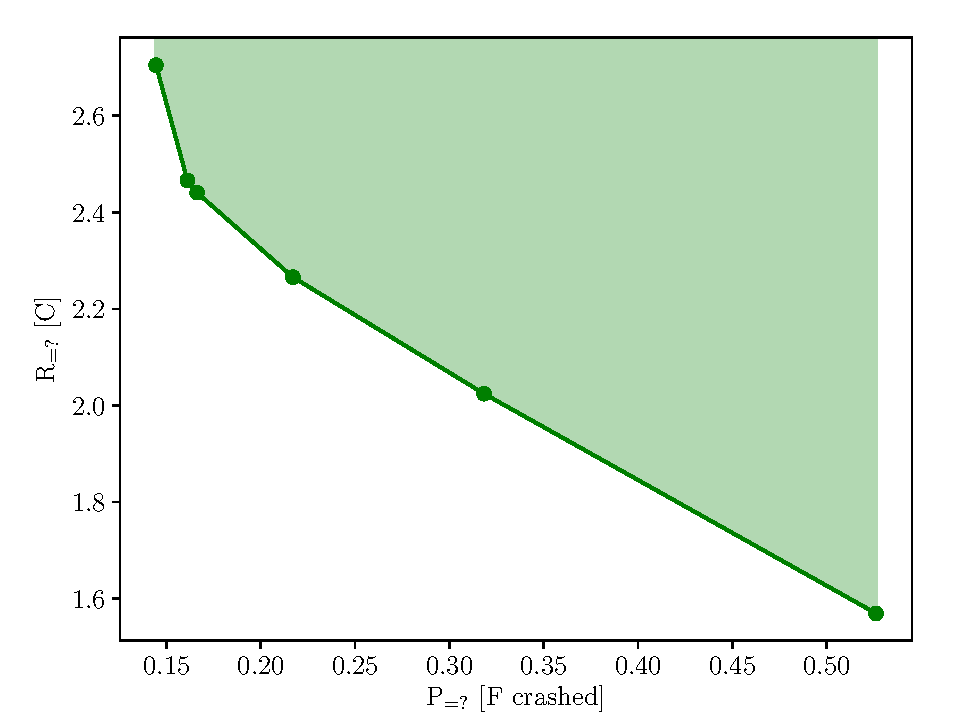
\includegraphics[width=0.75\textwidth]{results/additional/pareto.pdf}
\caption{Pareto curve for the model checking of the lane penalising property.}
\label{fig:lane_penalising_pareto}
\end{figure}

Observing this curve, it is possible to conclude that it is feasible to have \texttt{R<=1.8 [C]}, and thus the following property:

\begin{minipage}{\linewidth}
{\vspace{1em}
\begin{lstlisting}
multi(Pmin=? [F crashed], R<=1.8 [C])
\end{lstlisting}
}
\end{minipage}

yields an adversary which can be used to generate a sample path in the model. Similarly to what is presented in Section~\ref{sec:simulator}, a simulator was created to allow for the visualisation of a path in the model (the code for which is shown in Appendix~\ref{sec:strat_synth_and_sym}). The results of the simulation are presented in Figure~\ref{fig:lane_penalising_sim}.

\begin{figure}[H]
\centering
\begin{subfigure}{0.75\textwidth}
  \centering
  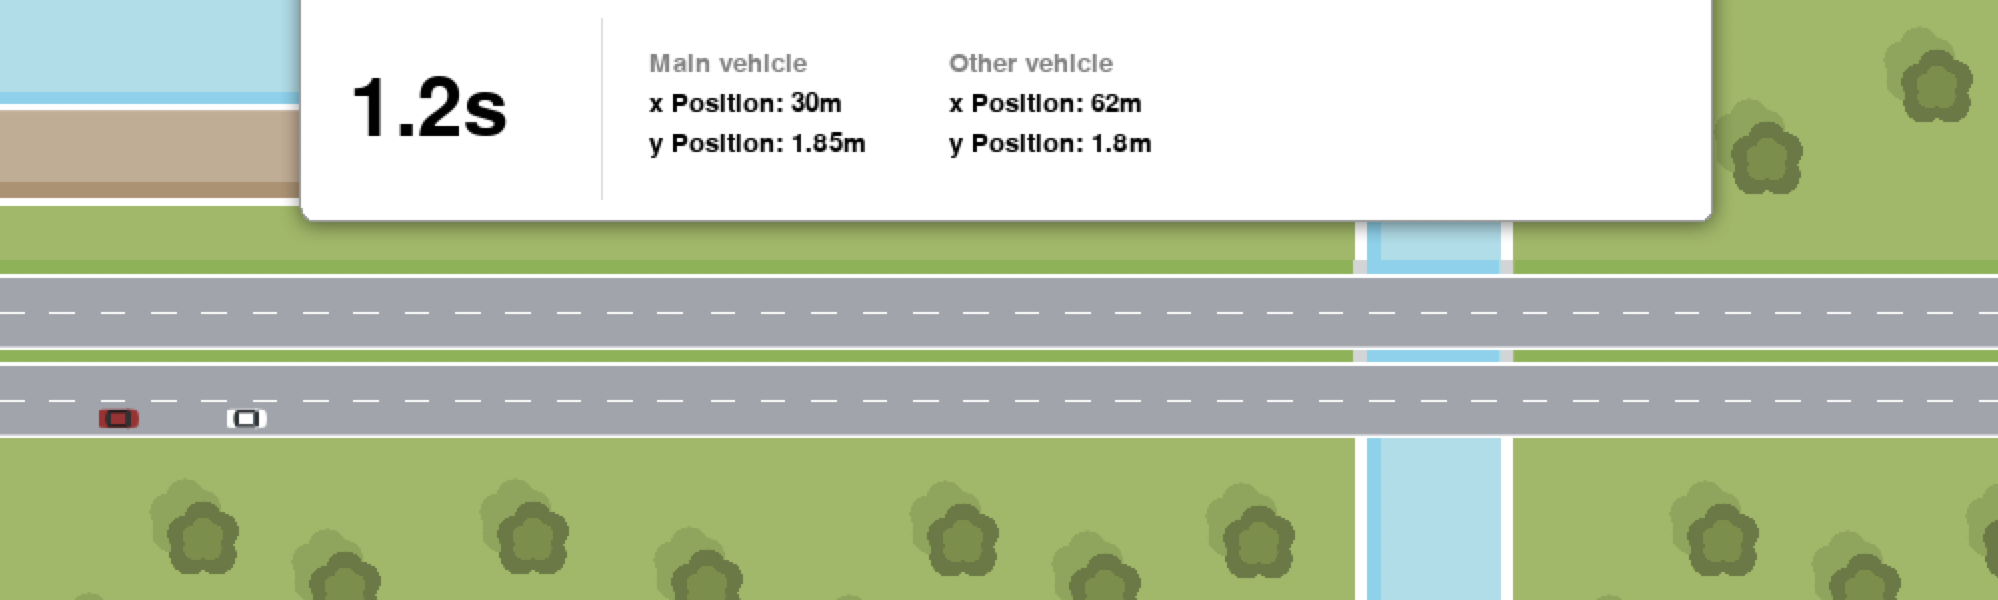
\includegraphics[width=1\textwidth]{results/additional/snap_1.png}
\end{subfigure}\\ \vspace{2px}
\begin{subfigure}{0.75\textwidth}
  \centering
  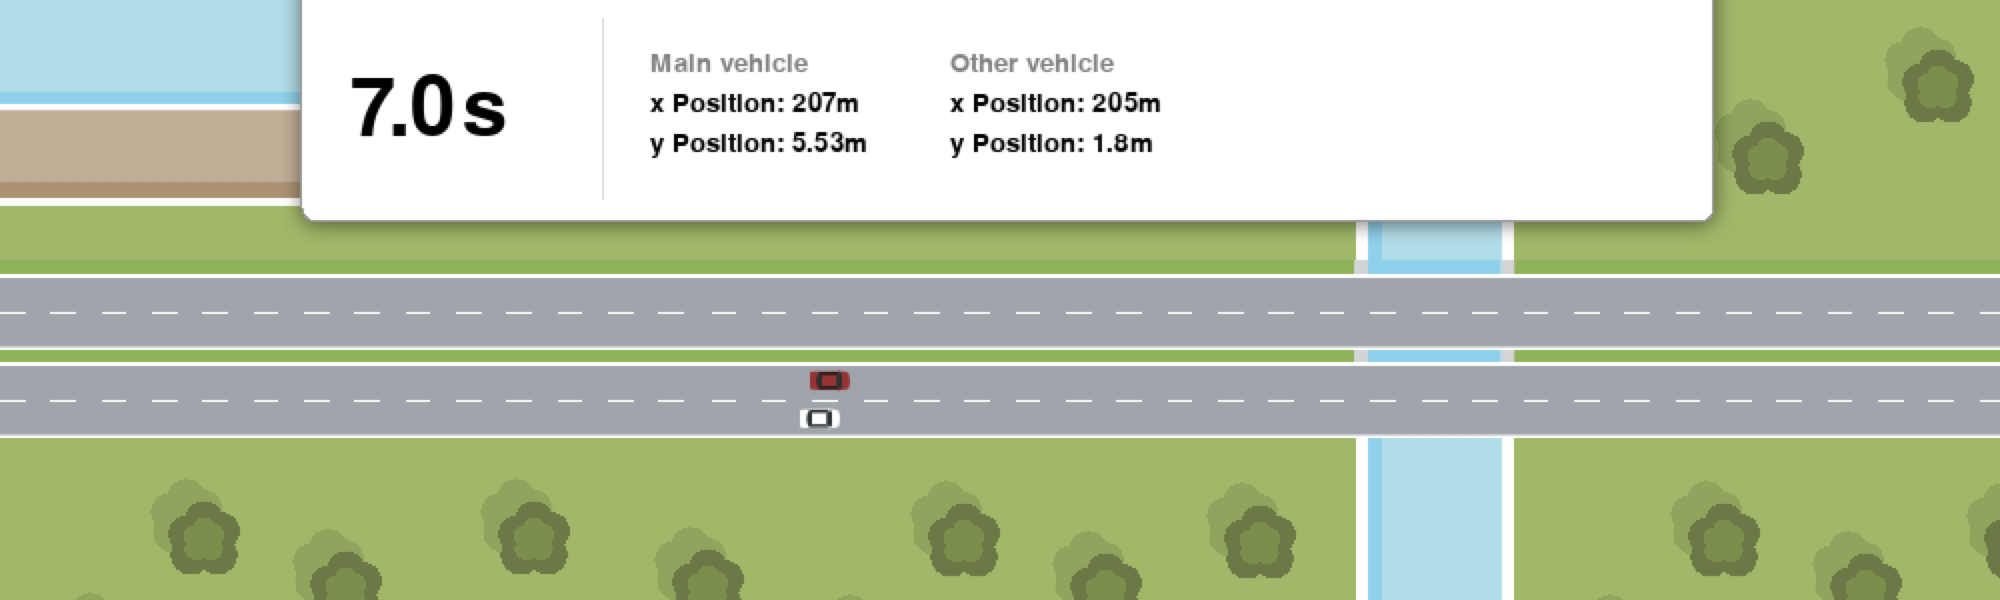
\includegraphics[width=1\linewidth]{results/additional/snap_2.png}
\end{subfigure} \\ \vspace{2px}
\begin{subfigure}{0.75\textwidth}
  \centering
  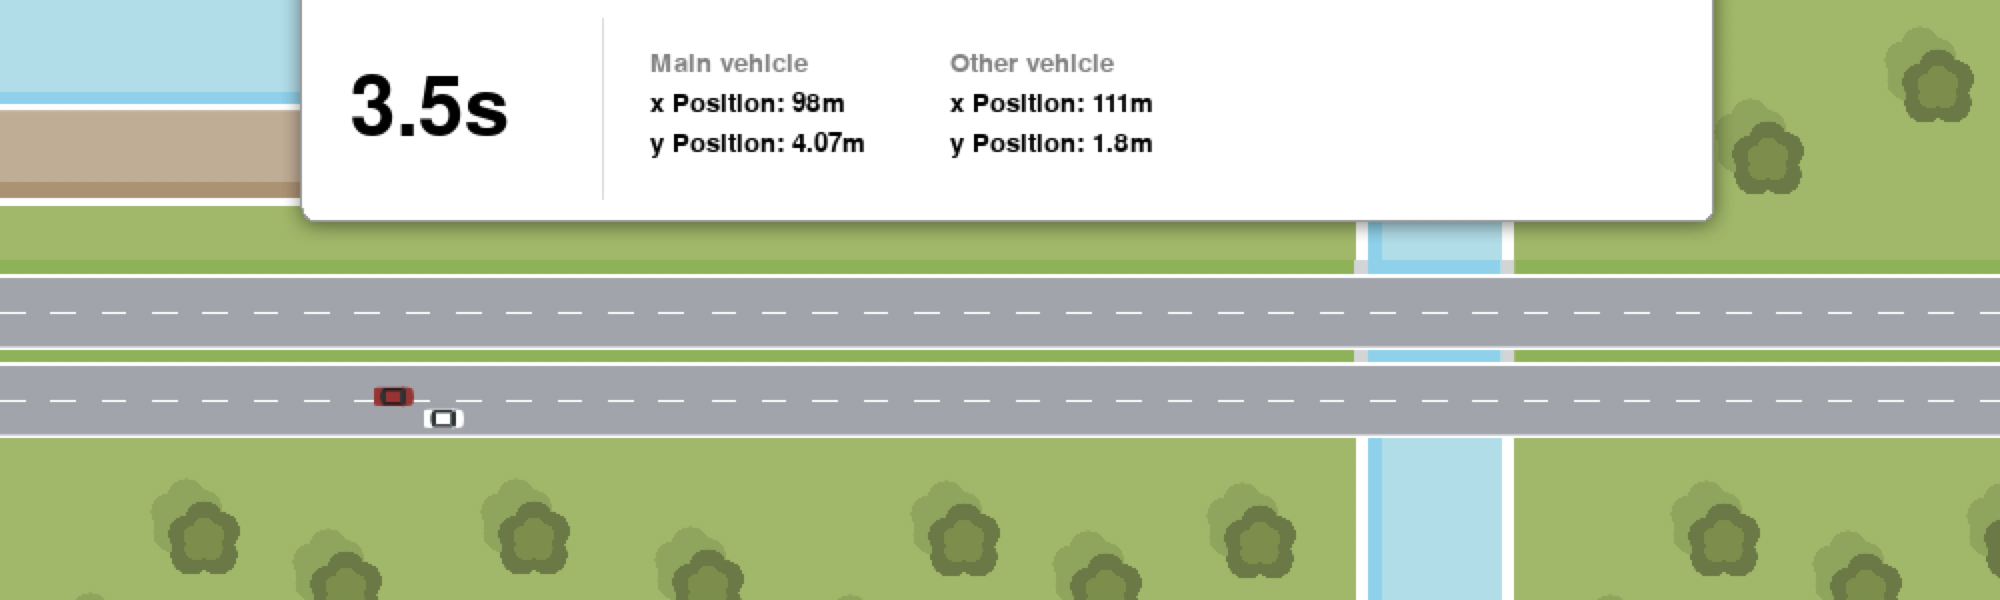
\includegraphics[width=1\linewidth]{results/additional/snap_3.png}
\end{subfigure} \\ \vspace{2px}
\begin{subfigure}{0.75\textwidth}
  \centering
  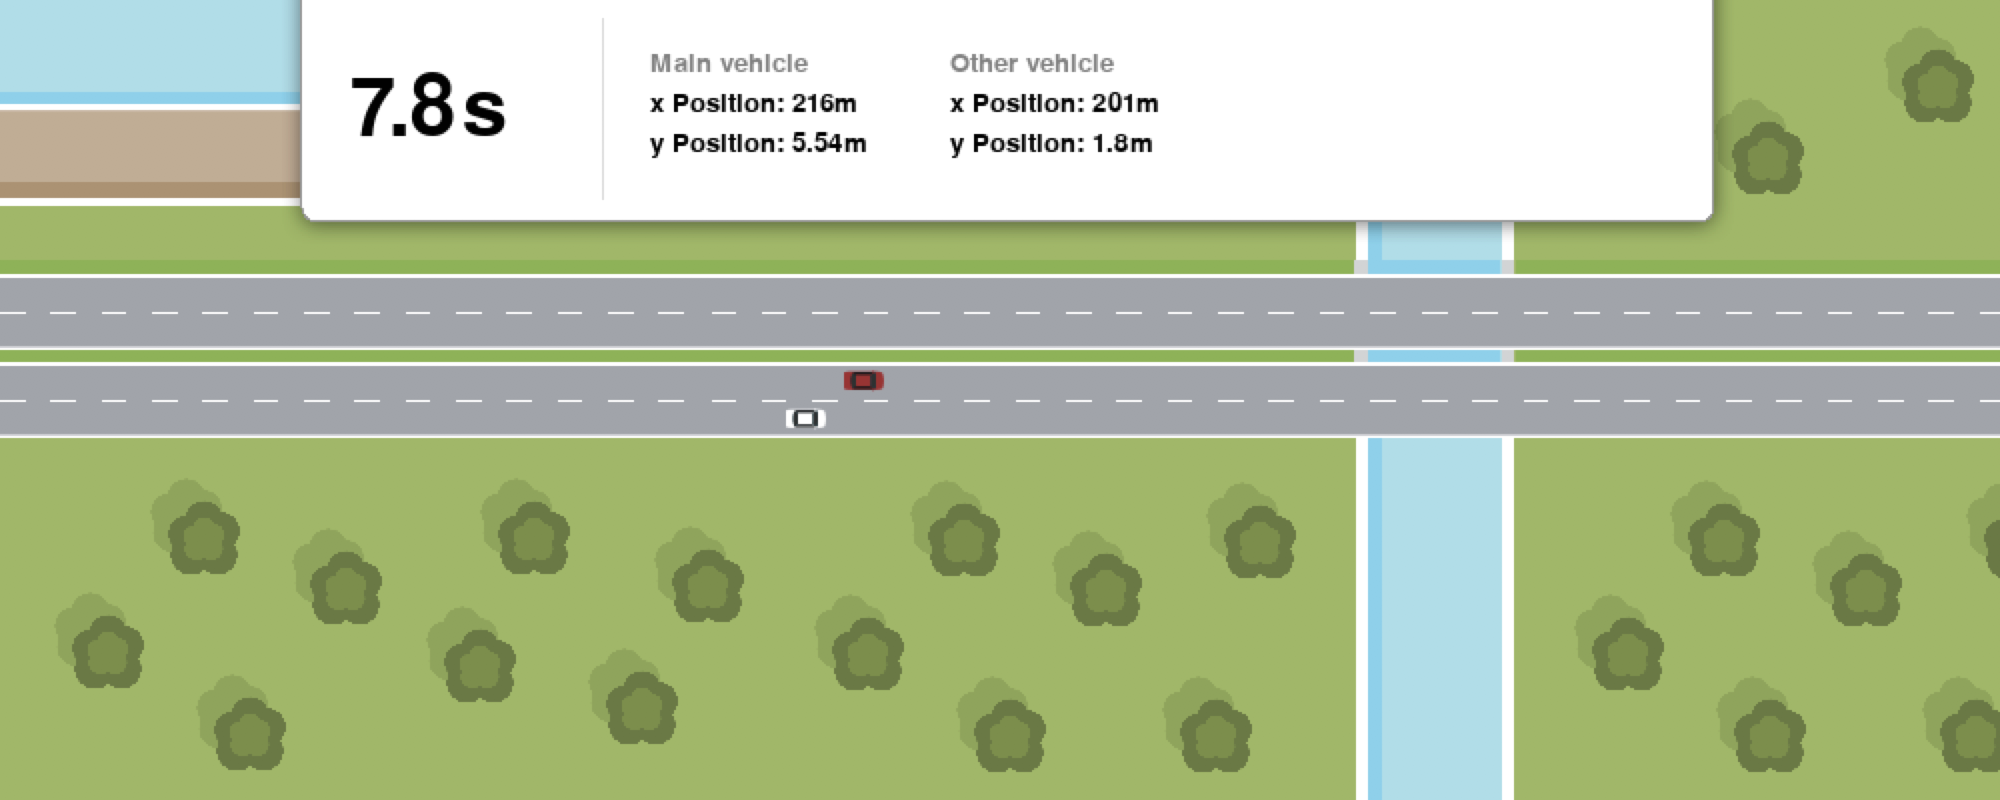
\includegraphics[width=1\linewidth]{results/additional/snap_4.png}
\end{subfigure} \\ \vspace{2px}
\begin{subfigure}{0.75\textwidth}
  \centering
  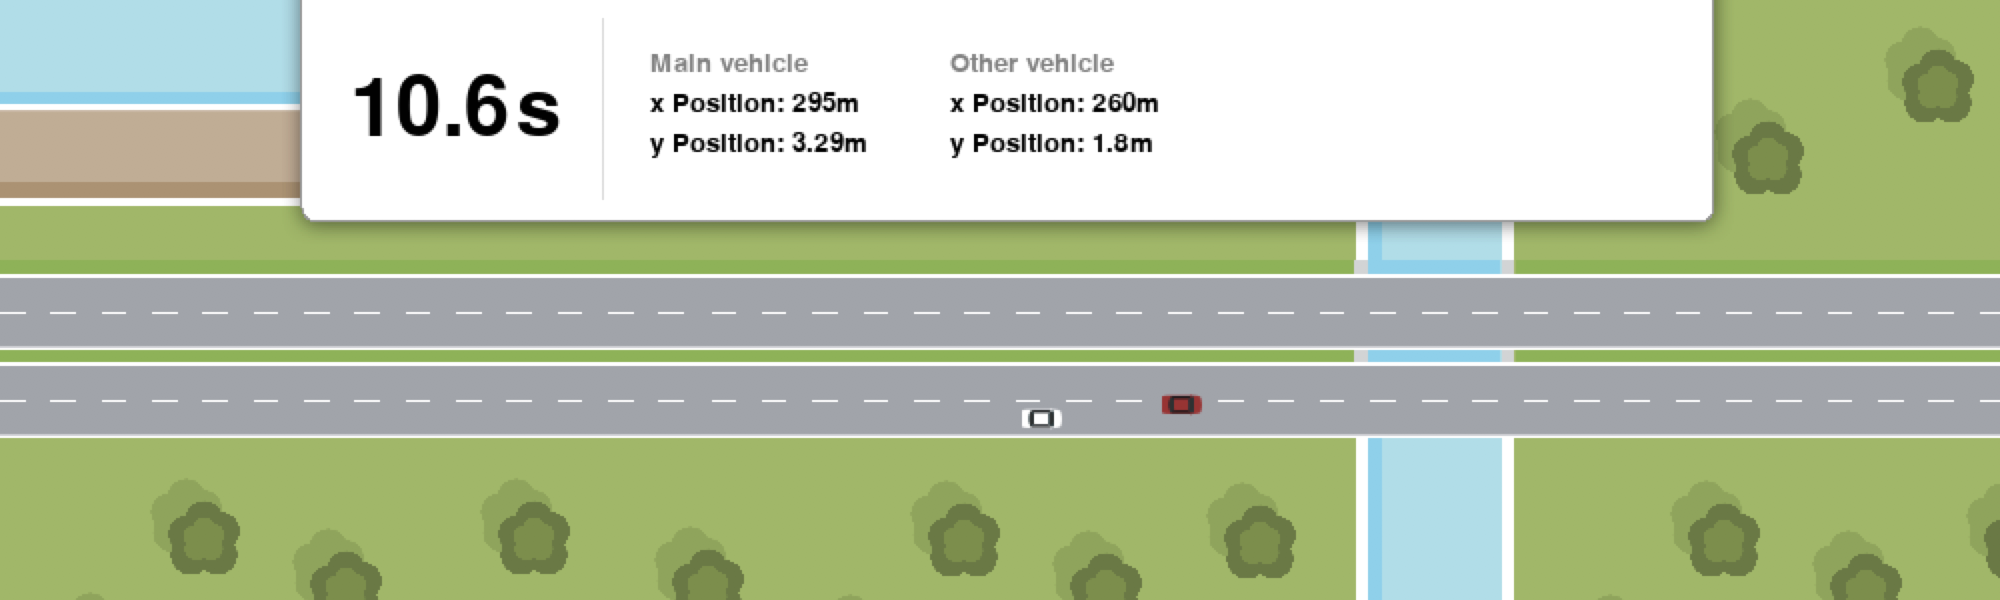
\includegraphics[width=1\linewidth]{results/additional/snap_5.png}
\end{subfigure} \\ \vspace{2px}
\begin{subfigure}{0.75\textwidth}
  \centering
  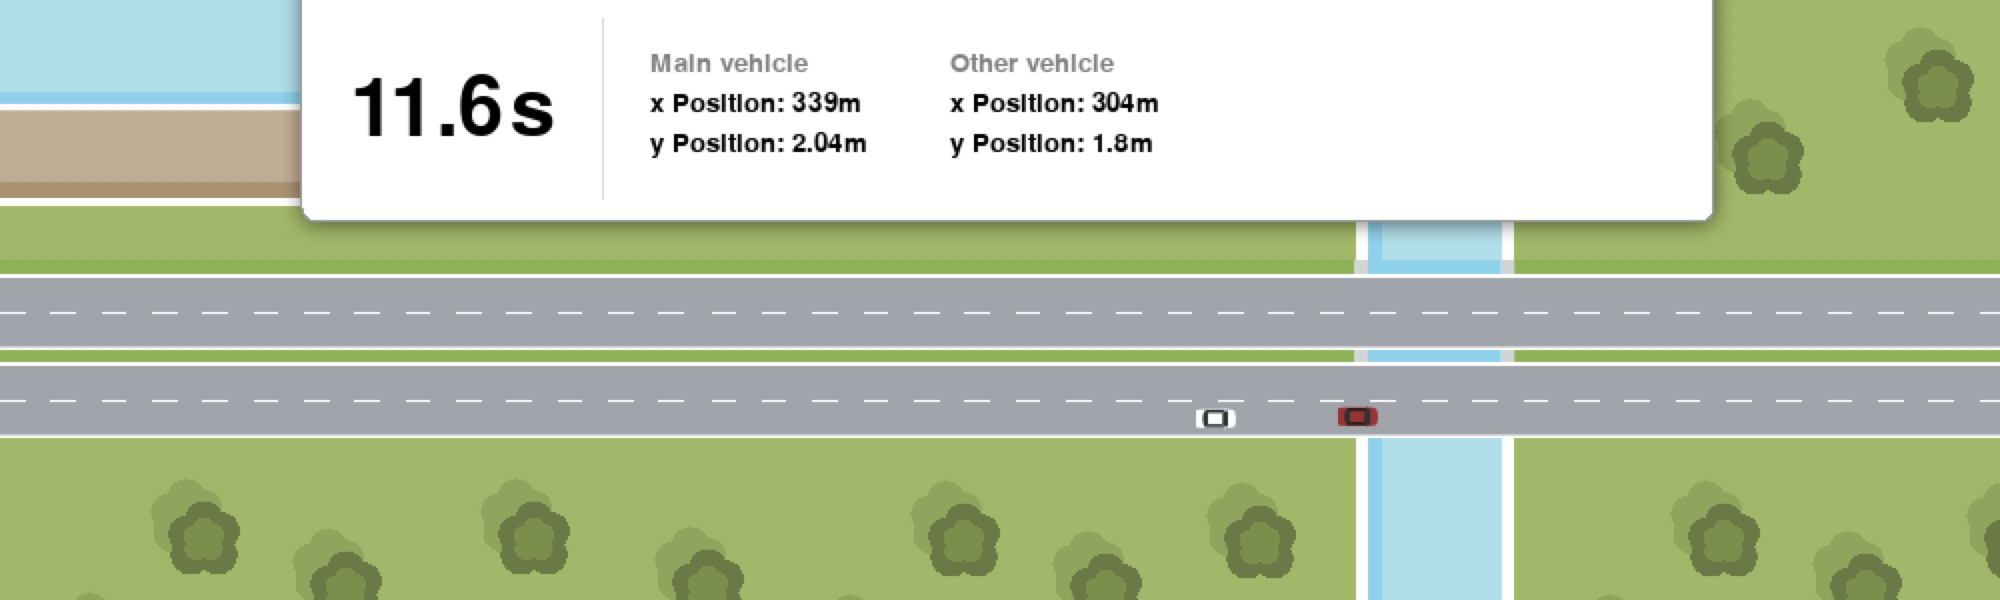
\includegraphics[width=1\linewidth]{results/additional/snap_6.png}
\end{subfigure}
\caption{Snapshots of the simulator for one of the paths of the model.}
\label{fig:lane_penalising_sim}
\end{figure}

As observed, minimal time is spent in the left lane, with the main vehicle returning to the right lane as soon as it passes the lead vehicle.

%\textbf{Three-objective Properties}
%
%In order to guarantee more than only safety and liveness in the model, an alternative to this would be to include multi-objective properties with more than 2 objectives. Such a property would have the format of the one below:
%
%\begin{minipage}{\linewidth}
%{\vspace{1em}
%\begin{lstlisting}
%multi(Pmin=? [F crashed], Pmax=? [F (x=length) & (t<T)], Rmin=? [C])
%\end{lstlisting}
%}
%\end{minipage}
%
%for a given constant $T$ and well defined reward structure. However, neither PRISM nor Storm allow for the model checking of these properties and the generation of the 3D Pareto curve they would entail.

\subsection{Unsafe by Construction}

Until this point, the assumption has been that the goal of the assistance system was to enforce safety and liveness. However, assume a bad actor has access to the model and the deployment process used in the vehicle. In such a case, it becomes important to evaluate the extent of the damage that such an actor could do. Take the same scenario as above, $(d_{type}, v, v_1, x_{1,0}) = (1, 30, 22, 50)$. Let's also assume that the bad actor wants the accident to happen after the the driver has driven between the $100$ and $200m$. The following property can be considered:

\begin{minipage}{\linewidth}
{\vspace{1em}
\begin{lstlisting}
multi(Pmax=? [F crashed], Pmax=? [x <= 100 U (x>100 & x<=200)])
\end{lstlisting}
}
\end{minipage}

which, when model checked, generates a Pareto curve of the trade-off between maximising the probability of crashing and the probability of reaching at least $100m$ and at most $200m$. The Pareto curve generated is presented in Figure~\ref{fig:unsafe_pareto}.

\begin{figure}[H]
\centering
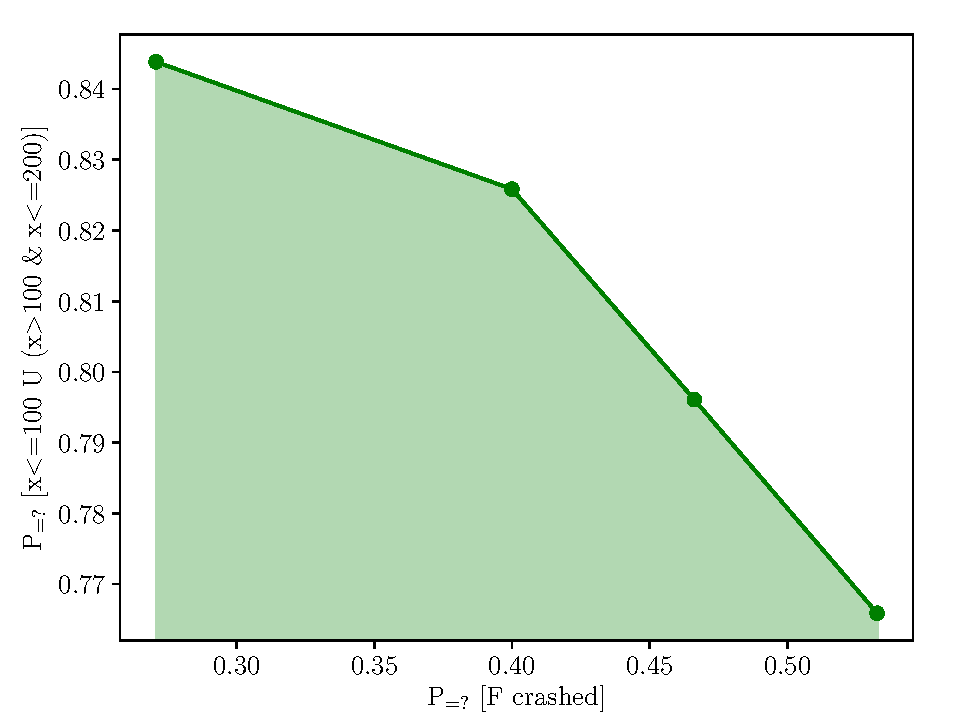
\includegraphics[width=0.75\textwidth]{results/additional/pareto_crashed.pdf}
\caption{Pareto curve for the model checking of the unsafe driving property.}
\label{fig:unsafe_pareto}
\end{figure}

By observing the Pareto curve, the following property can be devised:

\begin{minipage}{\linewidth}
{\vspace{1em}
\begin{lstlisting}
multi(Pmax=? [F crashed], P>=0.5 [x <= 100 U (x>100 & x<=200)])
\end{lstlisting}
}
\end{minipage}

This property maximises the probability of crashing, while requiring the vehicle to drive for at least $100m$ and at most $200m$ with probability at least 0.5 before the crash happens. By model checking this property, the maximum value of \texttt{P=? [F crashed]} comes out to be 0.5326, and the adversary obtained permits the generation of paths such as the one presented in the simulator frames in Figure~\ref{fig:unsafe_sim}. It should be noted that the value of \texttt{P=? [F crashed]} in the human driver model is 0.3935, and thus the bad actor has successfully increased the probability of crashing. 

\vspace{1em}
\begin{figure}[H]
\centering
\begin{subfigure}{0.75\textwidth}
  \centering
  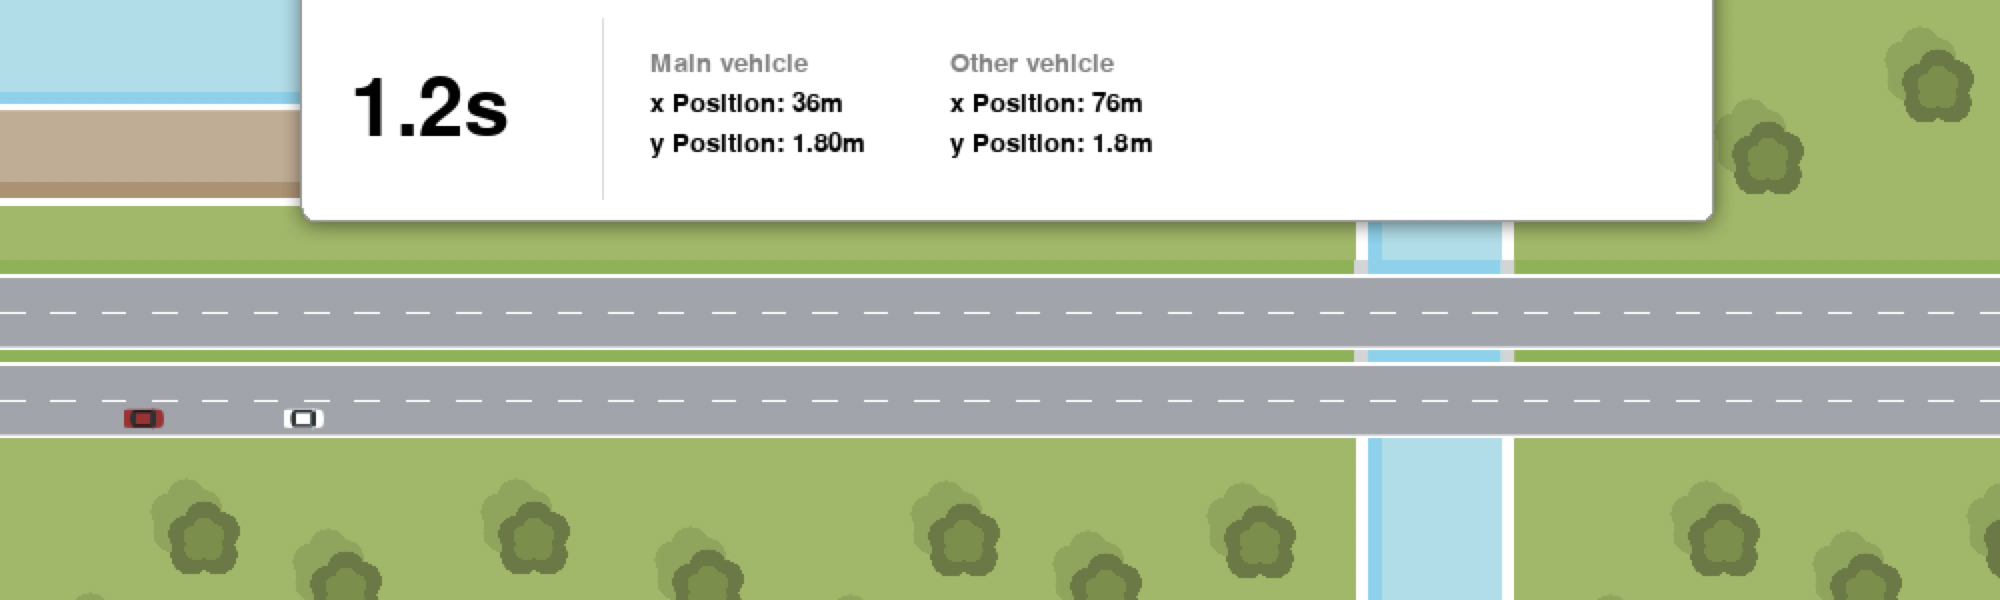
\includegraphics[width=1\textwidth]{results/additional/crash_1.png}
\end{subfigure}\\ \vspace{2px}
\begin{subfigure}{0.75\textwidth}
  \centering
  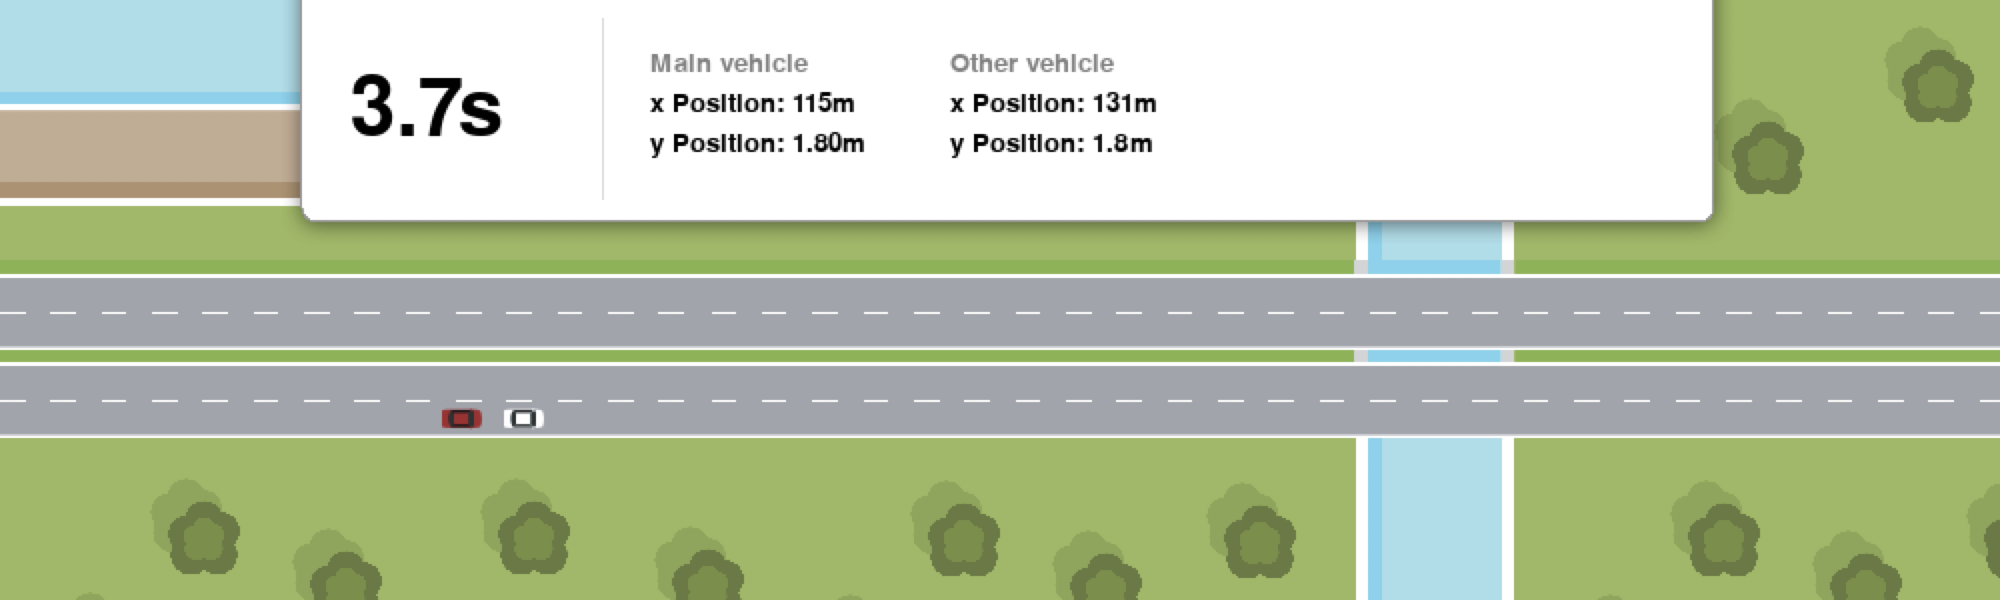
\includegraphics[width=1\linewidth]{results/additional/crash_2.png}
\end{subfigure} \\ \vspace{2px}
\begin{subfigure}{0.75\textwidth}
  \centering
  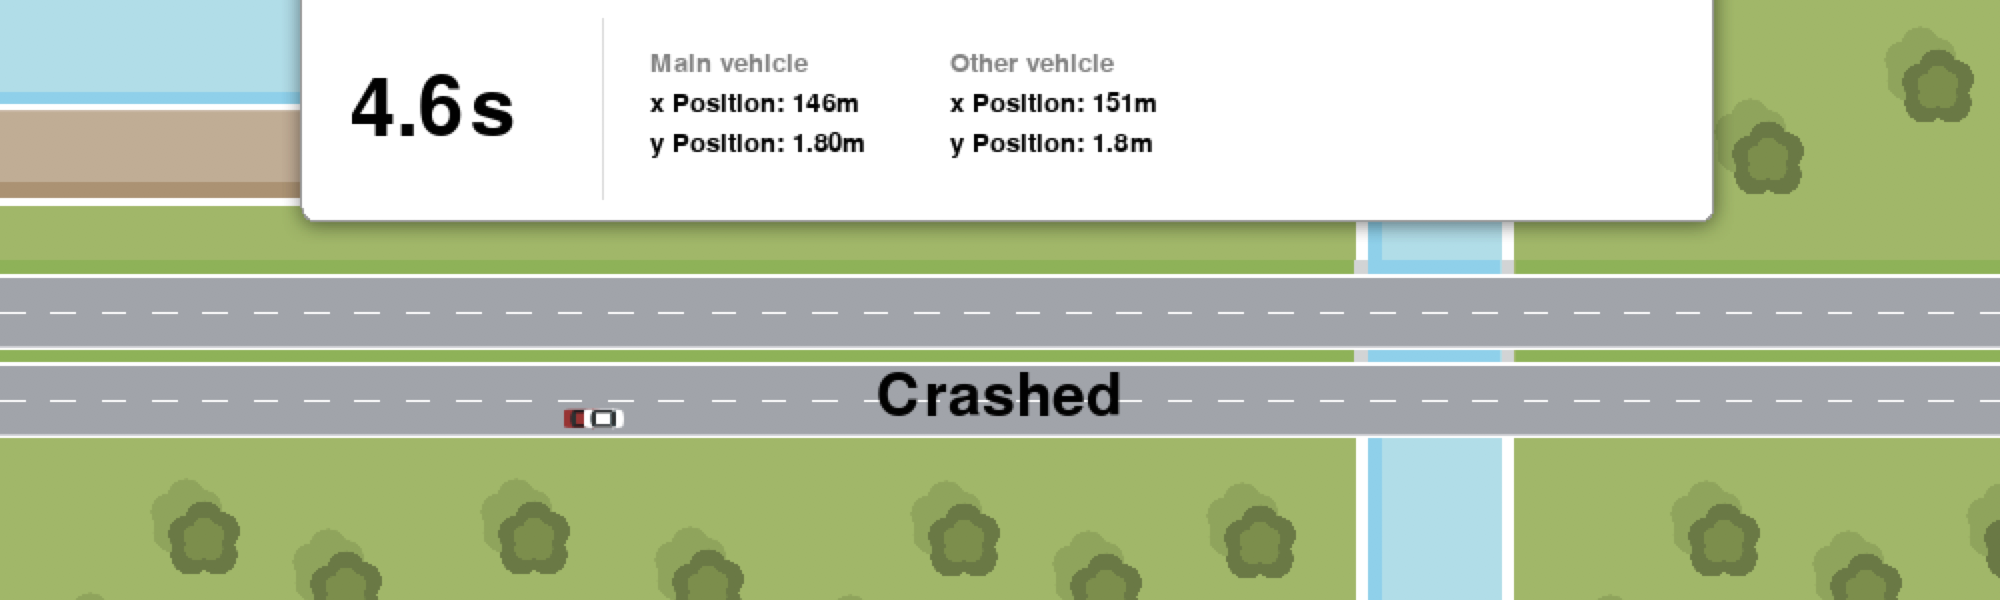
\includegraphics[width=1\linewidth]{results/additional/crash_3.png}
\end{subfigure}
\caption{Snapshots of the simulator for one of the paths of the model.}
\label{fig:unsafe_sim}
\end{figure}











